\documentclass{standalone}
\usepackage{PhysicalChemistryNote}
\begin{document}
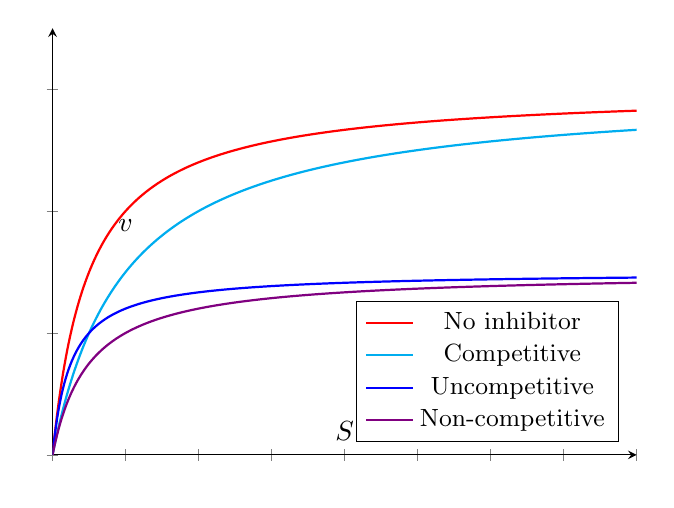
\begin{tikzpicture}
    \begin{axis}[
        width = 9cm,
        height = 7cm,
        legend pos = south east,
        x label style={at={(axis description cs:0.5,0.1)},anchor=north},
        y label style={at={(axis description cs:0.125,0.5)},rotate=270,anchor=south},
        xlabel = {$\con{S}$},
        ylabel = {$v$},
        axis lines = left,
        ymax = 3.5,
        domain = 0:8,
        samples = 400,
        xticklabels={},
        yticklabels={}
    ]
    \addplot [thick, red] {3/(1+0.5/x)};
    \addlegendentry{\small{No inhibitor}}
    \addplot [thick, cyan] {3/(1+1/x)};
    \addlegendentry{\small{Competitive}}
    \addplot [thick, blue] {3/(2+0.5/x)};
    \addlegendentry{\small{Uncompetitive}}
    \addplot [thick, violet] {3/(2+1/x)};
    \addlegendentry{\small{Non-competitive}}
    \end{axis}
\end{tikzpicture}
\end{document}